%!TEX root = ../dokumentation.tex

\chapter{Schnittstellenkommunikation}
In eingebetteten Systemen sind Sensoren und Aktoren erfolgt deren Anbindung oft mittels eines I\textsuperscript{2}C-Busses. Dies unterstützt Linux auf dem Raspberry Pi mit einem eigenen Subsystem. I\textsuperscript{2}C ist ein serieller Master-Slave-Datenbus, der über eine Datenleitung (SDA) und eine Taktleitung (SCL) verfügt und mit einer 7-Bit-Adresse 112 Geräte (Slaves) ansprechen kann. Für den Datenaustausch zwischen dem Raspberry Pi und dem ATMega8-Mikrocontroller kann man das I\textsuperscript{2}C/TWI-Übertragungsprotokoll nutzen.TWI steht für Two-Wire-Interface (TWI) und überträgt Daten seriell.
Beim Verbinden des AVR mit dem RPi muss darauf geachtet werden, dass der AVR mit 3,3V läuft, da ansonsten der Raspberry Pi beschädigt wird.\\
Im Anschluss daran muss der Raspberry Pi zur Kommunikation per I\textsuperscript{2}C als Master (Module hinzufügen und Installation des I\textsuperscript{2}C-Tools-Pakets) und der ATmega als I\textsuperscript{2}C-Slave vorbereitet werden. Außerdem muss die nötige I\textsuperscript{2}C-Bibliothek eingebunden werden.\\
Um die Verbindung herzustellen wird SDA und SCL des Raspberry (Pin 3 und 5) jeweils mit SDA und SCL des AVR verbunden. Dies entspricht beim ATmega8 Pin 27 und 28. Im nächsten Schritt werden die Leitungen über einen Pull-up-Widerstand mit Vcc verbunden.
Es muss dabei beachtet werden, dass der im Raspberry Pi verwendete Broadcomm BCM2835 Prozessor einen Fehler auslösen kann, der dazu führt, dass eine Kommunikation mit einigen I\textsuperscript{2}C Geräten unmöglich wird. In diesem Fall werden falsche Daten gelesen oder geschrieben. Der Grund hierfür ist, dass einige I\textsuperscript{2}C Geräte „clock stretching“ verwenden, welches nicht durch den Raspberry unterstützt wird. 

\section{Detaillierte Problembeschreibung}
Clock Stretching: Gemäß ihrer Spezifikation können I\textsuperscript{2}C-Slaves während einer Kommunikation die Clock-Leitung auf "low" halten. Auf Weise wird ein erneutes Steigen der Flanke verhindert und die Übertragung kann aktiv verzögert werden. Falls nötig ist so mehr Zeit für die Verarbeitung der Daten vorhanden. Gibt der I\textsuperscript{2}C die Clock Leitung dann wieder frei, ist es notwendig, dass der Master den Takt wieder an die Clock-Leitung anlegt.

Der eigentliche Fehler besteht also darin, dass die SCL Taktleitung nur maskiert wird sobald ein I\textsuperscript{2}C Slave die Taktleitung auf „low“ zieht. In der Folge stellt der Raspberry Pi allerdings nicht sicher, dass der folgende Takt die gleiche Länge besitzt. Es entstehen Spikes, die dann die Kommunikation mit dem I\textsuperscript{2}C Gerät unmöglich machen, da diese zu kurz sein können um vom I\textsuperscript{2}C-Slave erkannt zu werden. Das kann zu einer Verschiebung des Taktzyklus führen, sodass Master und Slave nicht mehr synchron laufen. \\
Dadurch entsteht ein weiteres Problem: der Raspberry liest die Datenleitung zu früh ein (noch während der Slave die Leitung auf „low“ hält) und selbst sehr kurze Clock-Stretching führen dazu, dass falsche Daten vom Raspberry gelesen werden.

Es gibt mehrere Möglichkeiten dieses Problem zu umgehen:
\begin{itemize}
	\item keine I\textsuperscript{2}C Geräte nutzen, die Clock-Stretching einsetzen
	\item clock-stretching nur am Ende nach dem Lesen des ACK/NACK verwenden, und ihn dabei um mindestens 1/2 Takt-Periode verlängern
	\item einen geringeren I\textsuperscript{2}C-Takt wählen, so dass die I\textsuperscript{2}C-Slaves schnell genug sind, und kein Clock-Stretching mehr benötigen
\end{itemize}
Im Rahmen dieser Arbeit wurde daher zunächst beschlossen, Clock-Stretching durch den I\textsuperscript{2}C-Slave zu unterbinden, da diese ohnehin nicht benötigt werden. Möglich wird dies durch Anpassungen in der Firmware (diese arbeitet nun mit Interrupts und daher viel schneller) und eine verringerte Frequenz am Raspberry.


\begin{figure}[H]
	\centering
	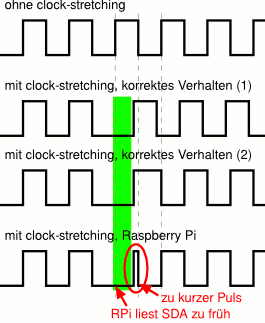
\includegraphics[scale=0.8]{images/rpi-i2c-bug.png}
	\caption{Clock-Stretching beim Raspberry Pi\footnotemark}
\end{figure}
\footnotetext{\url{http://www.advamation.de/technik/raspberrypi/rpi-i2c-bug.html}}

\section{Genutztes Protokoll}
Das erstellte Protokoll legt das Format, den Inhalt, die Bedeutung und die Reihenfolge gesendeter Nachrichten fest. Dies regelt den Ablauf und gleichzeitig wird eine Dokumentation darüber sichergestellt:
Es wird immer ein Byte gesendet. Dieses Byte repräsentiert einen Befehl:
Einzelheiten der vorhandenen Befehle 
(Gliederung: <Name> <Hex> <Beschreibung>)):
\begin{enumerate}
	\item PROT\_CONNECT 0x01: Verursacht einen Statuswechsel: Der Controller wartet auf die Messbefehle. Zusätzlich ist es mit Hilfe dieses Befehls möglich den Zustand des Controllers zurücksetzen.
	\item PROT\_DISCONNECT 0x02: Erneuter Statuswechsel: Controller kann nun selbstständig Messen und erwartet keine Befehle.
	\item PROT\_STARTMES 0x11: Befehl eine Laufzeitmessung zu starten, Ergebnis wird vom Mikrocontroller gepuffert.
	\item PROT\_DIST\_SEND 0x21: Sendet gleichzeitig ein Trigger-Signal und einen Ultraschallimpuls -> Wird von einem Controller ausgeführt um die Distanzen untereinander auszuessen.
	\item PROT\_DIST\_MES 0x22: Versetzt den Mikrocontroller in einen Wartezustand. Die Laufzeitmessung beginnt mit dem empfangenen Trigger-Signal. Das Ergebnis wird gepuffert. Das Kommando muss bei den beiden Controllern ausgeführt werden, bevor die dritte Platine das Kommando PROT\_DIST\_SEND erhält.
\end{enumerate}
Der Master (RPi) kann zu jedem Zeitpunkt Daten anfordern. Gesendet werden kann Folgendes:
\begin{enumerate}
	\item PROT\_MESSUCC 0x15: Wenn die Messung erfolgreich war, folgen 2 Byte (uint16) Messdaten in der Einheit mm. 
	\item PROT\_MESFAIL 0x16: Wenn die Messung fehlgeschlagen ist (kein Signal empfangen), folgen keine weiteren Daten.
	\item PROT\_NODATA 0x51: Dabei handelt es sich um einen Fehlercode: Der Controller verfügt über keinerlei Messdaten. Entweder wurde keine Messung gestartet, oder sie wurde noch nicht beendet.
\end{enumerate}
Die maximale Dauer einer Messung beträgt $66 ms$ ($2^{16} Bit / 1000000 Hz, 344m/s * 66ms = ca. 22m$). Diese Zeitspanne muss abgewartet werden, bis die Daten angefordert werden können und eine weitere Messung (anderer oder selber Controller) gestartet werden kann. Die drei Controller haben für den I\textsuperscript{2}C-Bus folgende Adressen abhängig von den Platinen fest zugeordnet: 0x2a, 0x2c, 0x2e.

